\documentclass[a4paper,10pt]{article}
\usepackage{amsmath}
\usepackage{amssymb}
\usepackage{graphicx}
\usepackage{hyperref}
\usepackage{listings}
\usepackage{xcolor}

% Definizione dei colori per i listati
\definecolor{mybackgroundcolor}{rgb}{0.95, 0.95, 0.95}
\definecolor{mykeywordcolor}{rgb}{0.9, 0.0, 0.0}

% Configurazione dell'ambiente lstlisting
\lstset{ 
    backgroundcolor=\color{mybackgroundcolor}, % Colore di sfondo
    basicstyle=\footnotesize\ttfamily, % Dimensione del font e tipo
    keywordstyle=\color{mykeywordcolor}, % Colore delle parole chiave
    commentstyle=\color{gray}, % Colore dei commenti
    stringstyle=\color{red}, % Colore delle stringhe
    frame=single, % Bordo attorno al listato
    breaklines=true, % Ritorno a capo automatico
    captionpos=b % Posizione della didascalia
}

\title{Miniguida Python per Studenti}
\author{Nome dell'Insegnante}
\date{\today}

\begin{document}

\maketitle

\tableofcontents
\newpage

\section{Introduzione}
Python è un linguaggio di programmazione versatile e potente, ideale per iniziare a programmare e per l'analisi dati. In questa guida, esploreremo la sintassi base, l'ambiente di sviluppo Google Colab, e alcuni elementi chiave di Python, NumPy e Matplotlib.

\section{Sintassi Base e Ambiente di Sviluppo Google Colab}
Google Colab è un ambiente di sviluppo integrato (IDE) basato su Jupyter Notebook, che permette di eseguire codice Python direttamente nel browser.

\subsection{Accedere a Google Colab}
1. Apri il browser e vai su \url{https://colab.research.google.com/}.
2. Accedi con il tuo account Google.
3. Crea un nuovo notebook cliccando su \textit{New Notebook}.

\subsection{Scrivere ed Eseguire Codice}
Nel notebook, puoi scrivere ed eseguire codice Python in celle. Per eseguire una cella, premi \textit{Shift+Enter}.

Esempio:
\begin{lstlisting}[language=Python]
print("Hello, World!")
\end{lstlisting}

\section{Elementi del Linguaggio Python}

\subsection{Variabili e Oggetti}
Le variabili in Python non richiedono dichiarazioni esplicite del tipo. Esempio:
\begin{lstlisting}[language=Python]
x = 10
y = "Ciao"
z = 3.14
\end{lstlisting}

\subsection{Stringhe}
Le stringhe sono delimitate da virgolette singole o doppie. Esempio:
\begin{lstlisting}[language=Python]
stringa = "Questa è una stringa"
\end{lstlisting}

\subsubsection{F-String}
Le f-string sono una funzionalità di Python che permette di inserire variabili all'interno delle stringhe in modo semplice e leggibile. Si utilizzano anteponendo una `f` alla stringa e racchiudendo le variabili tra parentesi graffe `{}`.

Esempio:
\begin{lstlisting}[language=Python]
nome = "Alice"
eta = 25
stringa = f"Il nome è {nome} e l'età è {eta} anni."
print(stringa)
\end{lstlisting}

In questo esempio, le variabili `nome` e `eta` sono incluse direttamente all'interno della stringa senza la necessità di concatenare manualmente o utilizzare metodi di formattazione complessi.

Esempio con espressioni:
\begin{lstlisting}[language=Python]
a = 10
b = 5
stringa = f"La somma di {a} e {b} è {a + b}."
print(stringa)
\end{lstlisting}

In questo caso, anche le espressioni possono essere valutate direttamente all'interno delle parentesi graffe.

\subsection{Costrutto di Selezione}
Il costrutto di selezione in Python usa le parole chiave \textit{if}, \textit{elif} e \textit{else}. Esempio:
\begin{lstlisting}[language=Python]
x = 5
if x > 0:
    print("x è positivo")
elif x == 0:
    print("x è zero")
else:
    print("x è negativo")
\end{lstlisting}

\subsection{Controllo di Flusso}
I controlli di flusso includono strutture come cicli e dichiarazioni condizionali.

\subsubsection{Indentazione}
Python utilizza l'indentazione per definire blocchi di codice. Ogni blocco deve essere indentato con lo stesso numero di spazi o tabulazioni. Esempio:
\begin{lstlisting}[language=Python]
x = 10
if x > 0:
    print("x è positivo")
    if x > 5:
        print("x è maggiore di 5")
\end{lstlisting}

\subsubsection{Cicli \textit{for}}
Il ciclo \textit{for} in Python è estremamente versatile e può essere utilizzato per iterare su una varietà di sequenze e strutture dati.

\paragraph{Iterare su una Lista}
Il ciclo \textit{for} può iterare attraverso ogni elemento di una lista. Esempio:
\begin{lstlisting}[language=Python]
frutti = ['mela', 'banana', 'ciliegia']
for frutto in frutti:
    print(frutto)
\end{lstlisting}

\paragraph{Iterare su un Range di Numeri}
Il ciclo \textit{for} può iterare attraverso un range di numeri generato dalla funzione \textit{range}. Esempio:
\begin{lstlisting}[language=Python]
for i in range(5):
    print(i)
\end{lstlisting}

\paragraph{Iterare su un Insieme}
Gli insiemi (\textit{sets}) sono collezioni non ordinate di elementi unici. Esempio:
\begin{lstlisting}[language=Python]
insieme = {1, 2, 3, 4}
for numero in insieme:
    print(numero)
\end{lstlisting}

\paragraph{Iterare su un Dizionario}
I dizionari (\textit{dict}) sono collezioni di coppie chiave-valore. Esempio di iterazione su chiavi e valori:
\begin{lstlisting}[language=Python]
dizionario = {'nome': 'Alice', 'età': 25, 'città': 'Roma'}

# Iterare sulle chiavi
for chiave in dizionario:
    print(chiave, dizionario[chiave])

# Iterare su chiavi e valori
for chiave, valore in dizionario.items():
    print(chiave, valore)
\end{lstlisting}

\paragraph{Enumerare gli Elementi di una Sequenza}
La funzione \textit{enumerate} restituisce una coppia (indice, valore) per ogni elemento di una sequenza. Esempio:
\begin{lstlisting}[language=Python]
frutti = ['mela', 'banana', 'ciliegia']
for indice, frutto in enumerate(frutti):
    print(indice, frutto)
\end{lstlisting}

\paragraph{Uso di \textit{zip} per Iterare su Più Sequenze}
La funzione \textit{zip} può essere utilizzata per iterare su più sequenze contemporaneamente. Esempio:
\begin{lstlisting}[language=Python]
nomi = ['Alice', 'Bob', 'Charlie']
eta = [25, 30, 35]

for nome, eta_persona in zip(nomi, eta):
    print(nome, eta_persona)
\end{lstlisting}

\subsubsection{Cicli \textit{while}}
Il ciclo \textit{while} itera finché una condizione è vera. È utile quando non si conosce in anticipo il numero di iterazioni. Ecco alcuni esempi:

\paragraph{Esempio Base}
Un ciclo `while` di base per contare da 0 a 4:
\begin{lstlisting}[language=Python]
count = 0
while count < 5:
    print(count)
    count += 1
\end{lstlisting}

\paragraph{Esempio con Lista}
In questo esempio, gli elementi della lista vengono rimossi uno alla volta fino a che la lista è vuota:
\begin{lstlisting}[language=Python]
lista = [1, 2, 3, 4, 5]
while lista:
    elemento = lista.pop(0)
    print(f"Eliminato: {elemento}, Lista rimanente: {lista}")
\end{lstlisting}

\section{Elementi di NumPy}

\subsection{Array}
NumPy è una libreria fondamentale per il calcolo scientifico in Python. Gli array NumPy sono simili alle liste, ma permettono operazioni matematiche vettorizate. Esempio:
\begin{lstlisting}[language=Python]
import numpy as np
arr = np.array([1, 2, 3, 4])
print(arr)
\end{lstlisting}

\subsection{Generazione di Array}
NumPy fornisce diverse funzioni per creare array. Esempio:
\begin{lstlisting}[language=Python]
zeros = np.zeros(5)
ones = np.ones(5)
range_arr = np.arange(10)
\end{lstlisting}

\subsection{Indicizzazione degli Array}
Gli elementi di un array possono essere accessi e modificati utilizzando gli indici. Esempio:
\begin{lstlisting}[language=Python]
arr = np.array([1, 2, 3, 4, 5])
print(arr[0])  # Primo elemento
print(arr[-1])  # Ultimo elemento
arr[0] = 10  # Modifica il primo elemento
\end{lstlisting}

\subsection{Matematica con gli Array}
NumPy permette di eseguire operazioni matematiche sugli array in modo semplice. Esempio:
\begin{lstlisting}[language=Python]
arr = np.array([1, 2, 3, 4])
print(arr + 2)
print(arr * 2)
print(np.sqrt(arr))
\end{lstlisting}

\subsection{Principali Funzioni Matematiche di NumPy}
NumPy offre molte funzioni matematiche utili per operare sugli array. Ecco alcune delle principali:

\subsubsection{Funzioni Trigonometriche}
\begin{lstlisting}[language=Python]
import numpy as np
angles = np.array([0, np.pi/2, np.pi])
print(np.sin(angles))  # Calcola il seno
print(np.cos(angles))  # Calcola il coseno
print(np.tan(angles))  # Calcola la tangente
\end{lstlisting}

\subsubsection{Funzioni Esponenziali e Logaritmiche}
\begin{lstlisting}[language=Python]
values = np.array([1, 2, 3])
print(np.exp(values))  # Calcola l'esponenziale
print(np.log(values))  # Calcola il logaritmo naturale
print(np.log10(values))  # Calcola il logaritmo in base 10
\end{lstlisting}

\subsubsection{Statistiche di Base}
\begin{lstlisting}[language=Python]
data = np.array([1, 2, 3, 4, 5])
print(np.mean(data))  # Media
print(np.median(data))  # Mediana
print(np.std(data))  # Deviazione standard
\end{lstlisting}

\subsubsection{Altre Funzioni Utili}
\begin{lstlisting}[language=Python]
values = np.array([-1, 2, -3])
print(np.abs(values))  # Valore assoluto
print(np.sqrt(values + 4))  # Radice quadrata (aggiungiamo 4 per evitare valori negativi)
print(np.sum(values))  # Somma degli elementi
print(np.prod(values))  # Prodotto degli elementi
\end{lstlisting}

\section{Elementi di Matplotlib}

\subsection{Grafici a Dispersione}
Matplotlib è una libreria per la creazione di grafici in Python. Esempio di grafico a dispersione:
\begin{lstlisting}[language=Python]
import matplotlib.pyplot as plt
import numpy as np

x = np.random.rand(50)
y = np.random.rand(50)

plt.scatter(x, y)
plt.title("Grafico a Dispersione")
plt.xlabel("X")
plt.ylabel("Y")
plt.savefig('grafico_dispersione.png')
plt.show()
\end{lstlisting}

Includi il grafico nel documento:
\begin{figure}[h!]
    \centering
    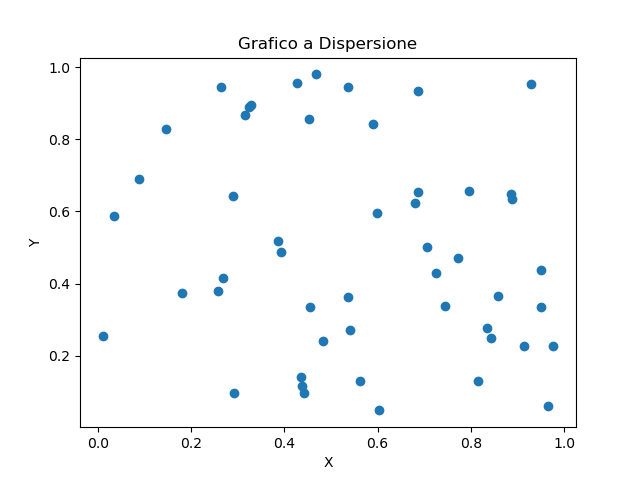
\includegraphics[width=0.8\textwidth]{grafico_dispersione.png}
    \caption{Grafico a Dispersione}
    \label{fig:dispersione}
\end{figure}

\subsection{Grafici con Barre di Errore}
I grafici con barre di errore mostrano l'incertezza nei dati. Esempio:
\begin{lstlisting}[language=Python]
import matplotlib.pyplot as plt
import numpy as np

x = np.linspace(0, 10, 10)
y = np.sin(x)
yerr = 0.2

plt.errorbar(x, y, yerr=yerr, fmt='-o')
plt.title("Grafico con Barre di Errore")
plt.xlabel("X")
plt.ylabel("Y")
plt.savefig('grafico_barre_errore.png')
plt.show()
\end{lstlisting}

Includi il grafico nel documento:
\begin{figure}[h!]
    \centering
    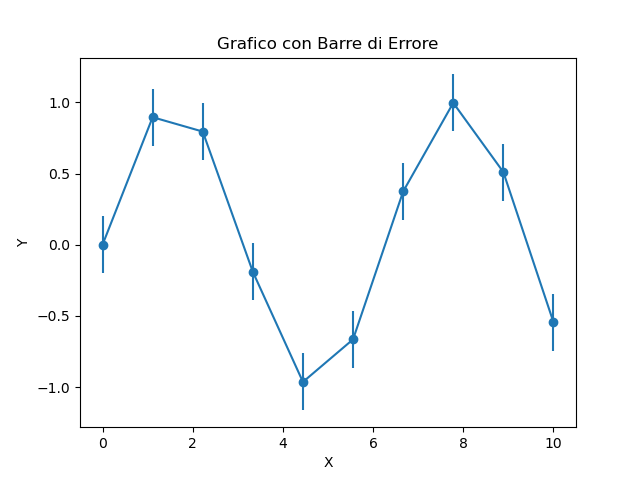
\includegraphics[width=0.8\textwidth]{grafico_barre_errore.png}
    \caption{Grafico con Barre di Errore}
    \label{fig:barre_errore}
\end{figure}

\subsection{Grafico Spazio-Tempo e Velocità-Tempo per Moto Uniforme a Tratti}
Consideriamo un moto uniforme a tratti, dove un oggetto si muove a tre diverse velocità in tre intervalli di tempo distinti. Creiamo due grafici: uno per il moto spaziale-temporale e uno per la velocità-tempo.

\subsubsection{Grafico Spazio-Tempo}
Nel grafico spazio-tempo, mostriamo il percorso dell'oggetto in funzione del tempo. Supponiamo che l'oggetto abbia velocità costanti di 2 m/s, 4 m/s e 6 m/s nei rispettivi intervalli di tempo.

Esempio di codice:
\begin{lstlisting}[language=Python]
import matplotlib.pyplot as plt
import numpy as np

# Dati
tempi = [0, 2, 5, 8, 10]
posizioni = [0, 4, 16, 28, 40]

# Creazione del grafico
plt.figure(figsize=(12, 6))
plt.plot(tempi, posizioni, marker='o')
plt.title("Grafico Spazio-Tempo per Moto Uniforme a Tratti")
plt.xlabel("Tempo (s)")
plt.ylabel("Posizione (m)")
plt.grid(True)
plt.savefig('grafico_spazio_temporale.png')
plt.show()
\end{lstlisting}

\subsubsection{Grafico Velocità-Tempo}
Il grafico velocità-tempo mostra la variazione della velocità in funzione del tempo. Ogni intervallo di tempo corrisponde a una velocità costante.

Esempio di codice:
\begin{lstlisting}[language=Python]
import matplotlib.pyplot as plt
import numpy as np

# Dati
tempi = [0, 2, 5, 8, 10]
velocita = [2, 2, 4, 4, 6]

# Creazione del grafico
plt.figure(figsize=(12, 6))
plt.step(tempi, velocita, where='post', marker='o')
plt.title("Grafico Velocità-Tempo per Moto Uniforme a Tratti")
plt.xlabel("Tempo (s)")
plt.ylabel("Velocità (m/s)")
plt.grid(True)
plt.savefig('grafico_velocita_temporale.png')
plt.show()
\end{lstlisting}

\subsubsection{Spiegazione dei Grafici}
\begin{itemize}
    \item \textbf{Grafico Spazio-Tempo:} Questo grafico mostra come la posizione dell'oggetto cambia nel tempo. È possibile osservare che il grafico è composto da segmenti lineari, ognuno con una pendenza diversa, che rappresenta le diverse velocità. L'area sotto la curva corrisponde alla distanza percorsa.
    \item \textbf{Grafico Velocità-Tempo:} Questo grafico mostra come la velocità cambia nel tempo. Utilizzando un grafico a passo, ogni intervallo di tempo mostra una velocità costante. Il grafico indica chiaramente le transizioni tra le diverse velocità.
\end{itemize}

Includi i grafici nel documento:
\begin{figure}[h!]
    \centering
    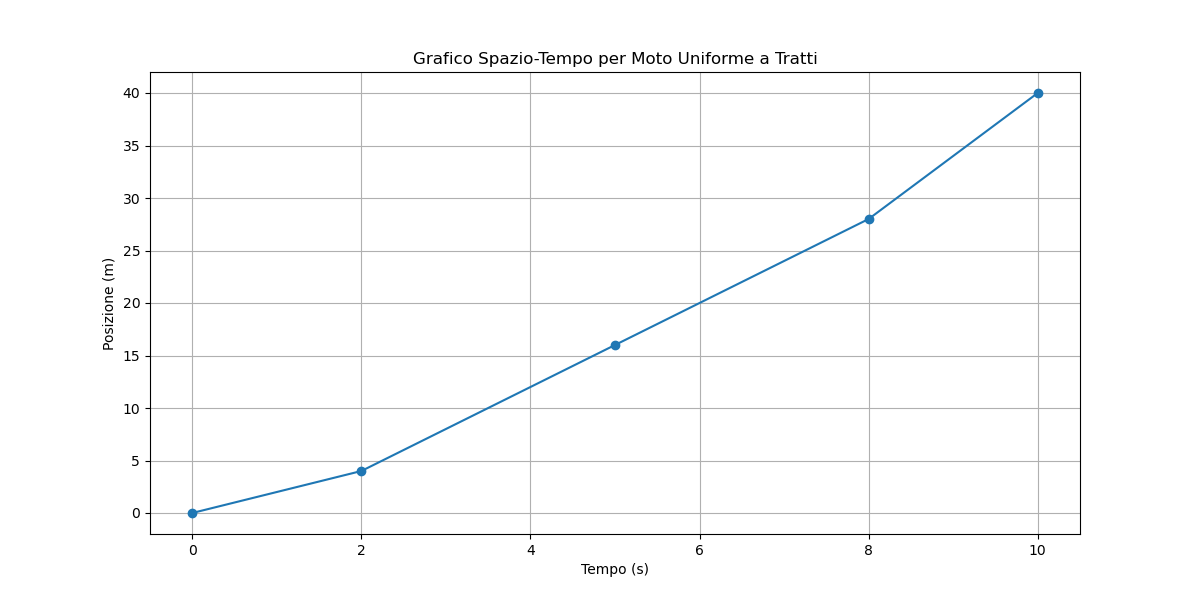
\includegraphics[width=0.8\textwidth]{grafico_spazio_temporale.png}
    \caption{Grafico Spazio-Tempo per Moto Uniforme a Tratti}
    \label{fig:spazio_temporale}
\end{figure}

\begin{figure}[h!]
    \centering
    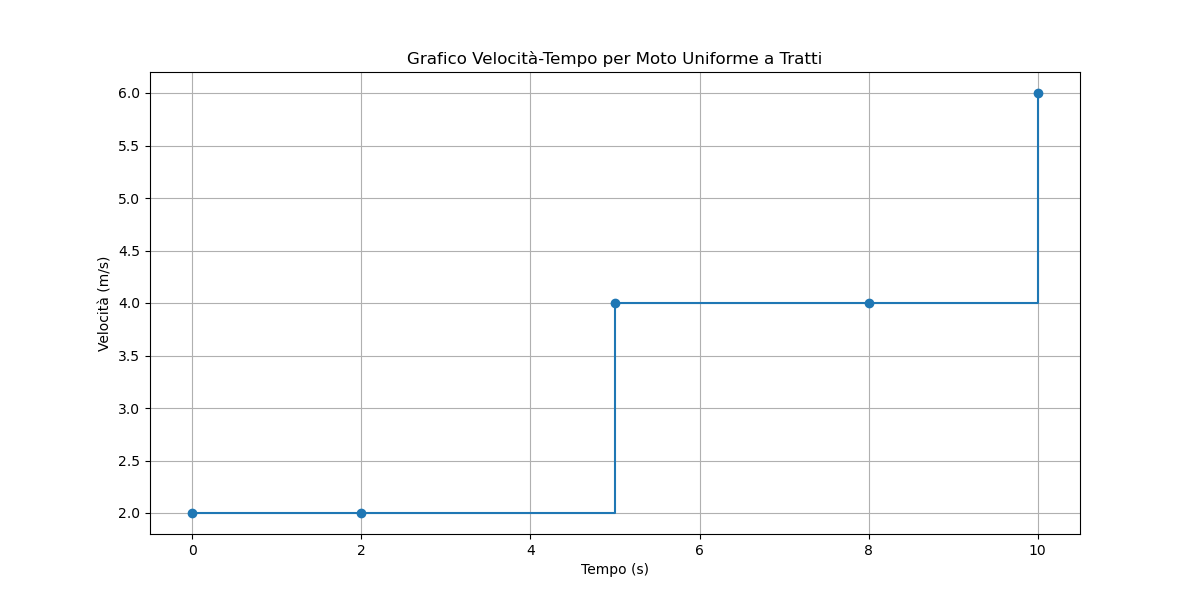
\includegraphics[width=0.8\textwidth]{grafico_velocita_temporale.png}
    \caption{Grafico Velocità-Tempo per Moto Uniforme a Tratti}
    \label{fig:velocita_temporale}
\end{figure}

\subsection{Grafico Altezza-Diametro di un Cilindro con Volume Fisso}
Infine, consideriamo un grafico che mostra come l'altezza di un cilindro varia in funzione del diametro della base, mantenendo fisso il volume.

Esempio di codice:
\begin{lstlisting}[language=Python]
import matplotlib.pyplot as plt
import numpy as np

# Costanti
volume = 1000  # Volume costante del cilindro in m³

# Diametro della base
diametro = np.linspace(1, 10, 100)  # Diametro varia da 1 a 10 metri

# Calcolo dell'altezza
altezza = volume / (np.pi * (diametro / 2)**2)

# Creazione del grafico
plt.figure(figsize=(12, 6))
plt.plot(diametro, altezza, label='Altezza = Volume / (π × (Diametro / 2)²)', color='green')
plt.title("Grafico dell'Altezza in Funzione del Diametro di Base (Volume Fisso)")
plt.xlabel("Diametro della Base (m)")
plt.ylabel("Altezza (m)")
plt.grid(True)
plt.legend()
plt.savefig('grafico_altezza_diametro.png')
plt.show()
\end{lstlisting}

Includi il grafico nel documento:
\begin{figure}[h!]
    \centering
    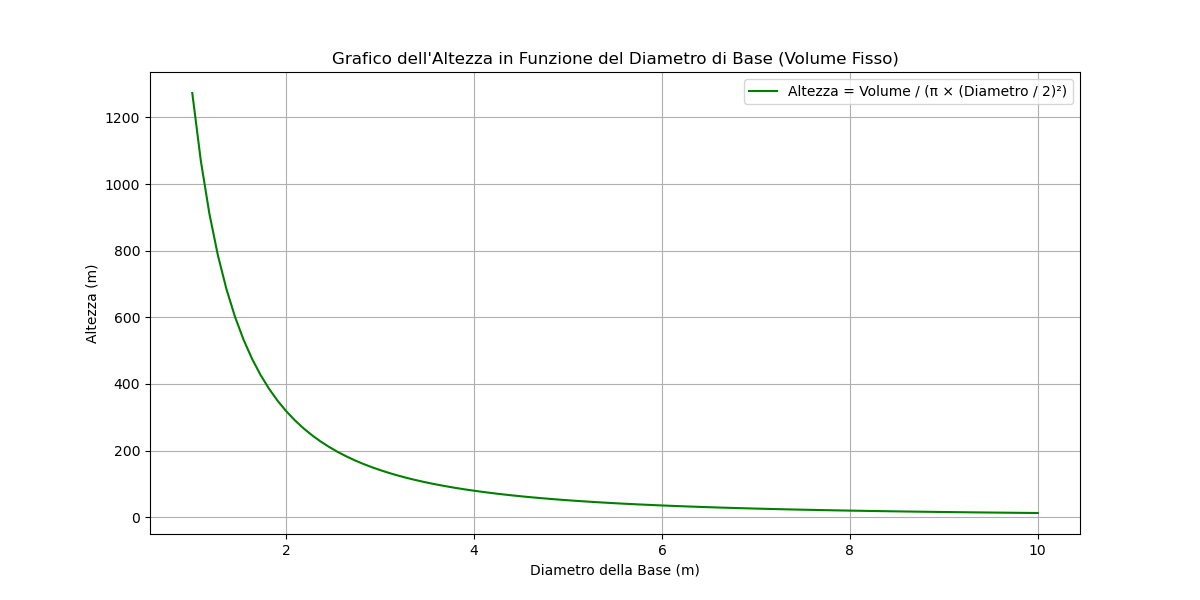
\includegraphics[width=0.8\textwidth]{grafico_altezza_diametro.png}
    \caption{Grafico dell'Altezza in Funzione del Diametro di Base (Volume Fisso)}
    \label{fig:altezza_diametro}
\end{figure}

\end{document}
